\documentclass{article}

\usepackage{hyperref}
\usepackage[T1]{fontenc}
\usepackage{graphicx}
\usepackage{float}
\usepackage[utf8]{inputenc}


\title{%
Laboratorium 3\\
  \huge Interpolacja}
\author{Mateusz Król}
\date{20/03/2024 r.}

\begin{document}
\maketitle


\section*{Zadanie 1.}
\textbf{Populacja Stanów Zjednoczonych na przestrzeni lat przedstawiała
się następująco:}
\begin{center}
  \begin{tabular}{c c} 
   Rok & Populacja\\
   1900 & 76 212 168\\
   1910 & 92 228 496\\
   1920 & 106 021 537\\
   1930 & 123 202 624\\
   1940 & 132 164 569\\
   1950 & 151 325 798\\
   1960 & 179 323 175\\
   1970 & 203 302 031\\
   1980 &226 542 199
  \end{tabular}
\end{center}
\textbf{Istnieje dokładnie jeden wielomian ósmego stopnia, który interpoluje
 powyższe dziewięć punktów, natomiast sam wielomian może być reprezentowany na różne sposoby.}
\\\\
Dla każdej z macierzy Vandermonde'a powstałych na podstawie zbiorów funkcji 
bazowych $\phi$:
$$ \phi_j(t) = t^{j-1}\mbox{, dla } j = 1,\dots,9$$
$$ \phi_j(t) = (t-1900)^{j-1}\mbox{, dla } j = 1,\dots,9$$
$$ \phi_j(t) = (t-1940)^{j-1}\mbox{, dla } j = 1,\dots,9$$
$$ \phi_j(t) = \left(\frac{t-1940}{40}\right)^{j-1} \mbox{, dla } j = 1,\dots,9$$
, współczynniki uwarunkowania wynosiły:
\begin{center}
  \begin{tabular}{  |c|c|c| } 
   \hline
   base function & $cond(V)$\\
   \hline
   $\phi_1$ & $3.98 \cdot 10^{32}$ \\
   \hline
   $\phi_2$ & $6.31 \cdot 10^{15}$ \\
   \hline
   $\phi_3$ & $9.32 \cdot 10^{12}$ \\
   \hline
   $\phi_4$ & $1.61 \cdot 10^{3}$ \\
   \hline
  \end{tabular}
\end{center}
Najlepiej uwarunkowaną bazą wielomianów jest
ta zbudowana na podstawie zbioru funkcji $\phi_j(t) = \left(\frac{t-1940}{40}\right)^{j-1}$.
\\\\
Korzystając z tej bazy i wykorzystując schemat \textit{Hornera}, 
obliczyłem wartości wielomianu interpolacyjnego na przedziale $[1900; 1990]$:
\begin{figure}[H]
  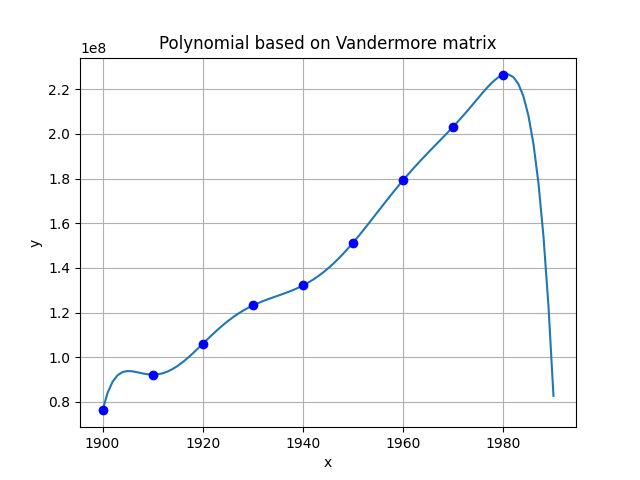
\includegraphics[width=\linewidth]{figures/vandermore.png}
\end{figure}
Na podstawie obliczonego wielomianu interpolacyjnego, wartość dla roku
1990 wynosi $\approx 82 749 141$, co w stosunku do prawdziwej wartości,
równej $248 709 873$, daje błąd względny na poziomie $\approx 66.73\%$.
\\\\
Wielomian interpolacyjny \textit{Lagrange}'a:
\begin{figure}[H]
  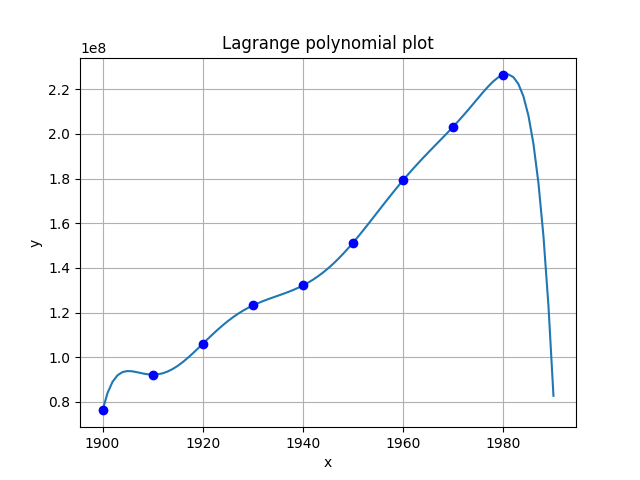
\includegraphics[width=\linewidth]{figures/lagrange.png}
\end{figure}
Wielomian interpolacyjny \textit{Newton}'a:
\begin{figure}[H]
  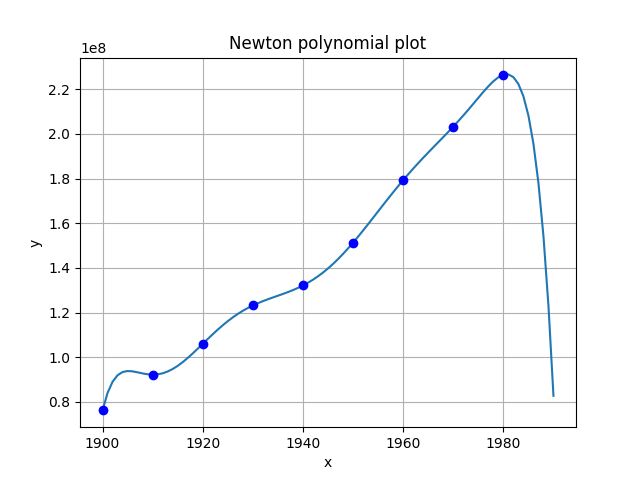
\includegraphics[width=\linewidth]{figures/newton.png}
\end{figure}
Po zaokrągleniu danych populacji dla każdego roku w tabeli, wciąż wykorzystując 
najlepiej uwarunkowaną bazę funkcji $\phi$, otrzymujemy następujący 
wielomian interpolacyjny:
\begin{figure}[H]
  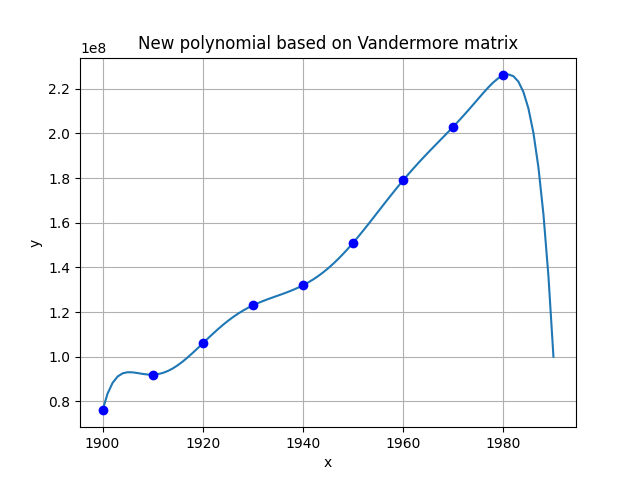
\includegraphics[width=\linewidth]{figures/new_vandermore.png}
\end{figure}

\subsection*{Wnioski}
\null\quad Pomimo zupełnie różnych sposobów reprezentacji wielomianu, 
wykresy prezentują się dokładnie tak samo. \\
\null\quad Zaokrąglenie danych populacji w podpunkcie (g), 
doprowadziło do otrzymania mniejszego błędu względnego ekstrapolowanej 
wartości dla roku 1990. Błąd spadł z $\approx 66.7\%$ do $\approx 59.8\%$.

\section*{Źródła}
\begin{itemize}
    \item \url{https://en.wikipedia.org/wiki/Newton_polynomial}
    \item \url{https://heath.cs.illinois.edu/scicomp/notes/cs450_chapt07.pdf}
\end{itemize}


\end{document}